\documentclass{standalone}
\usepackage{tikz}
\usetikzlibrary{patterns}
\usetikzlibrary{positioning}
\usetikzlibrary{patterns, positioning}
\usetikzlibrary{shapes.misc}
\usepackage[outline]{contour}
\contourlength{1.5pt} 
\usepackage[sfdefault]{ClearSans}

\begin{document}
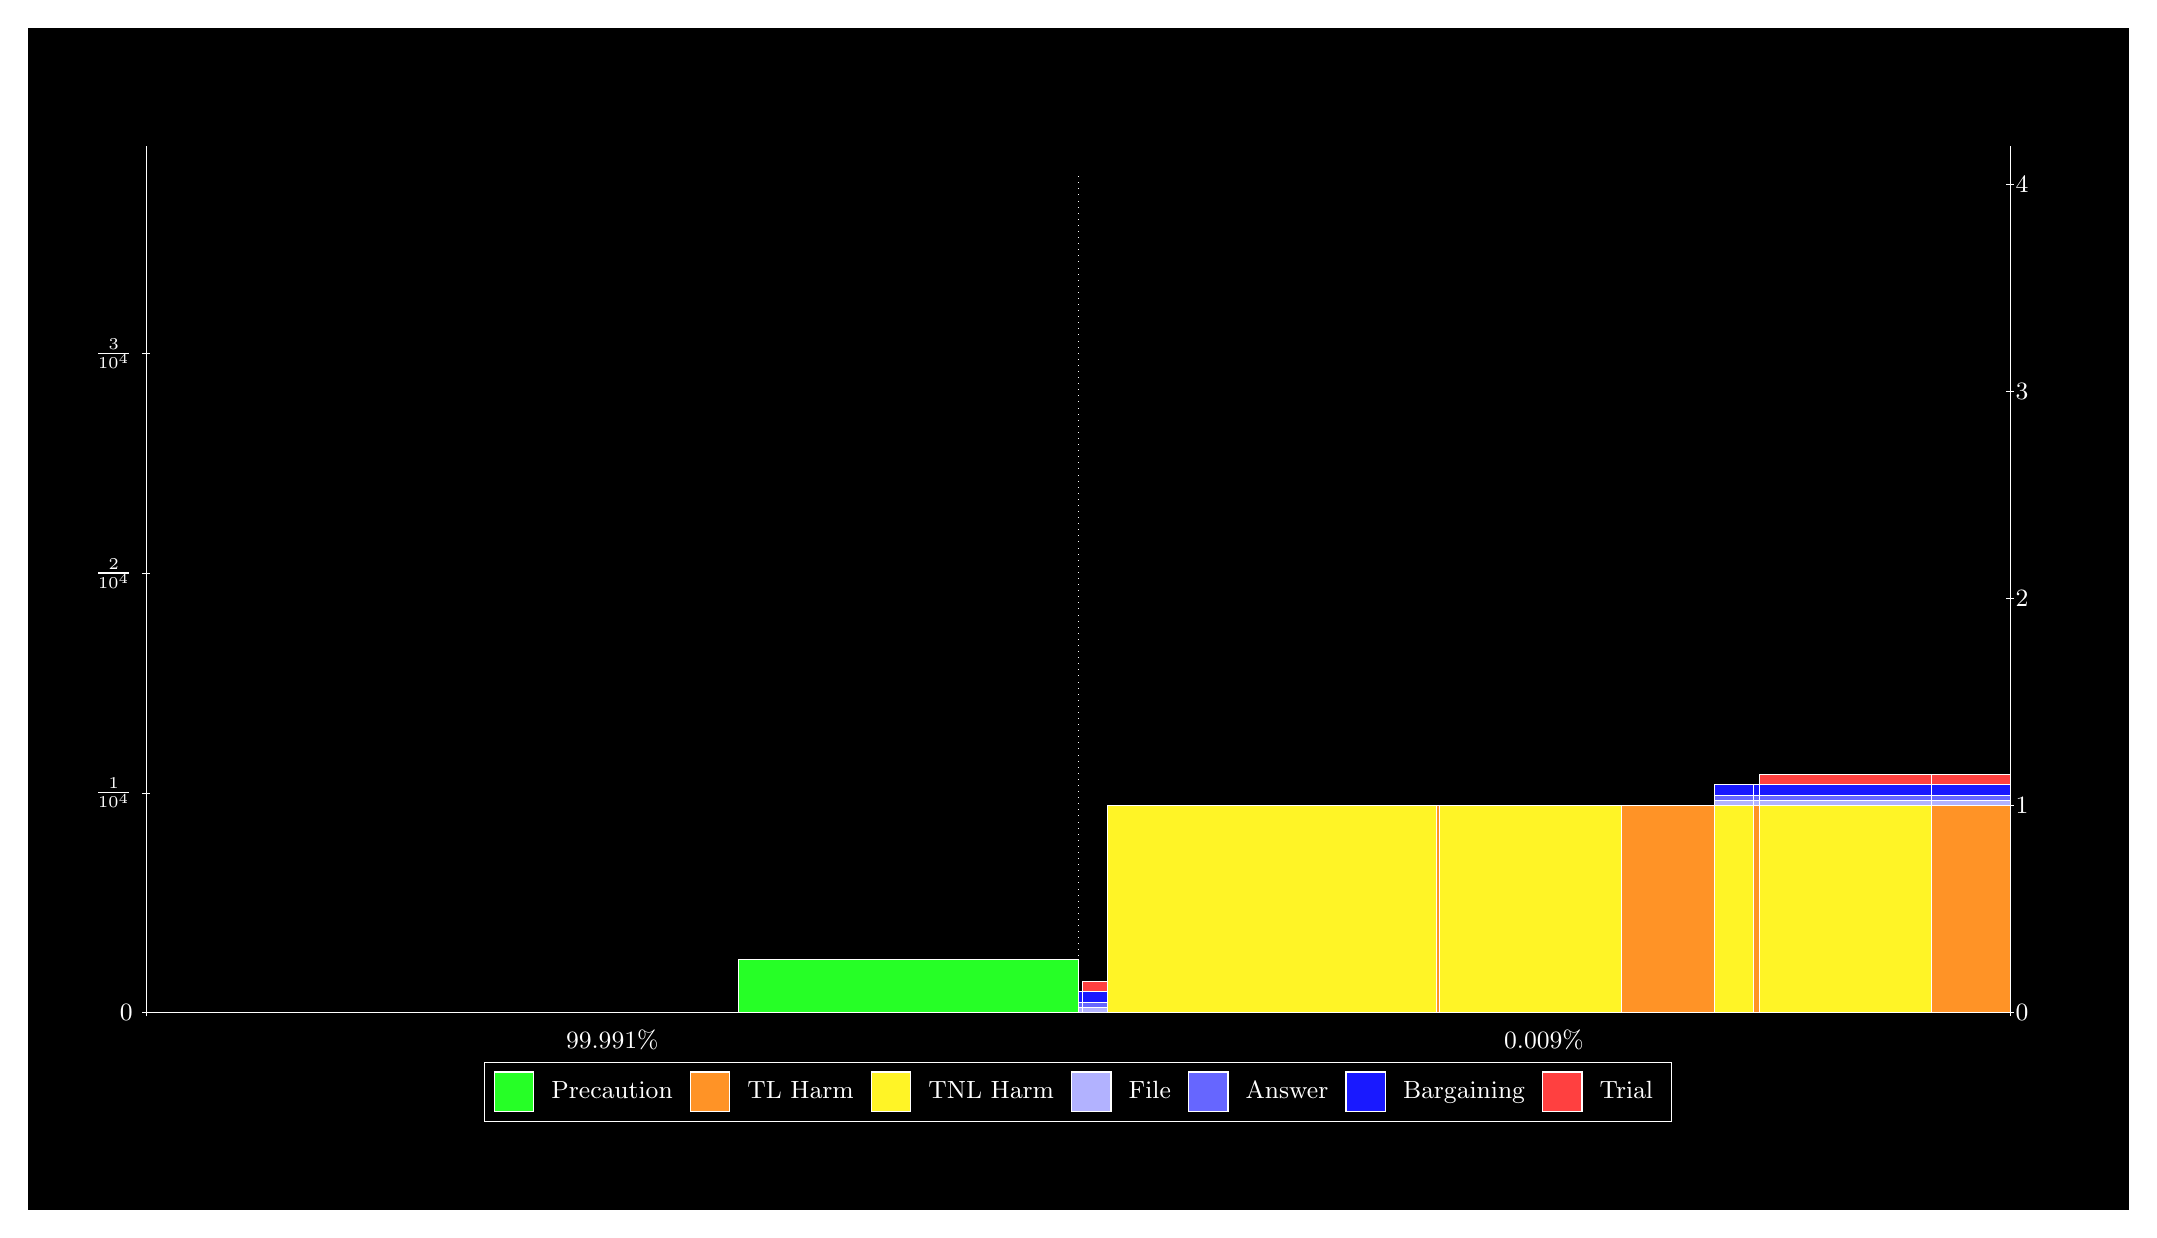
\begin{tikzpicture}
\draw[fill=black] (0,0) rectangle (26.667,15);
\draw[fill=green!85,draw=white,very thin] (9.0126,2.5) rectangle (13.333,3.1693);
\draw[fill=blue!30,draw=white,very thin] (13.333,2.5) rectangle (13.391,2.5658);
\draw[fill=blue!60,draw=white,very thin] (13.333,2.5658) rectangle (13.391,2.6315);
\draw[fill=blue!90,draw=white,very thin] (13.333,2.6315) rectangle (13.391,2.763);
\draw[fill=blue!30,draw=white,very thin] (13.391,2.5) rectangle (13.709,2.5658);
\draw[fill=blue!60,draw=white,very thin] (13.391,2.5658) rectangle (13.709,2.6315);
\draw[fill=blue!90,draw=white,very thin] (13.391,2.6315) rectangle (13.709,2.763);
\draw[fill=red!75,draw=white,very thin] (13.391,2.763) rectangle (13.709,2.8946);
\draw[fill=yellow!85,draw=white,very thin] (13.709,2.5) rectangle (17.877,5.1303);
\draw[fill=orange!85,draw=white,very thin] (17.877,2.5) rectangle (17.916,5.1303);
\draw[fill=green!85,draw=white,very thin] (17.916,2.5) rectangle (20.235,2.5001);
\draw[fill=yellow!85,draw=white,very thin] (17.916,2.5001) rectangle (20.235,5.1304);
\draw[fill=green!85,draw=white,very thin] (20.235,2.5) rectangle (21.408,2.5001);
\draw[fill=orange!85,draw=white,very thin] (20.235,2.5001) rectangle (21.408,5.1304);
\draw[fill=yellow!85,draw=white,very thin] (21.408,2.5) rectangle (21.904,5.1303);
\draw[fill=blue!30,draw=white,very thin] (21.408,5.1303) rectangle (21.904,5.1961);
\draw[fill=blue!60,draw=white,very thin] (21.408,5.1961) rectangle (21.904,5.2619);
\draw[fill=blue!90,draw=white,very thin] (21.408,5.2619) rectangle (21.904,5.3934);
\draw[fill=orange!85,draw=white,very thin] (21.904,2.5) rectangle (21.986,5.1303);
\draw[fill=blue!30,draw=white,very thin] (21.904,5.1303) rectangle (21.986,5.1961);
\draw[fill=blue!60,draw=white,very thin] (21.904,5.1961) rectangle (21.986,5.2619);
\draw[fill=blue!90,draw=white,very thin] (21.904,5.2619) rectangle (21.986,5.3934);
\draw[fill=yellow!85,draw=white,very thin] (21.986,2.5) rectangle (24.168,5.1303);
\draw[fill=blue!30,draw=white,very thin] (21.986,5.1303) rectangle (24.168,5.1961);
\draw[fill=blue!60,draw=white,very thin] (21.986,5.1961) rectangle (24.168,5.2619);
\draw[fill=blue!90,draw=white,very thin] (21.986,5.2619) rectangle (24.168,5.3934);
\draw[fill=red!75,draw=white,very thin] (21.986,5.3934) rectangle (24.168,5.5249);
\draw[fill=orange!85,draw=white,very thin] (24.168,2.5) rectangle (25.167,5.1303);
\draw[fill=blue!30,draw=white,very thin] (24.168,5.1303) rectangle (25.167,5.1961);
\draw[fill=blue!60,draw=white,very thin] (24.168,5.1961) rectangle (25.167,5.2619);
\draw[fill=blue!90,draw=white,very thin] (24.168,5.2619) rectangle (25.167,5.3934);
\draw[fill=red!75,draw=white,very thin] (24.168,5.3934) rectangle (25.167,5.5249);
\draw[white,very thin] (1.5,2.5) -- (1.5,13.5);
\draw[white,very thin] (1.45,2.5) -- (1.55,2.5);
\node[font=\small,text=white, anchor=east] at (1.45, 2.5) {0};
\draw[white,very thin] (1.45,5.2886) -- (1.55,5.2886);
\node[font=\small,text=white, anchor=east] at (1.45, 5.2886) {$\frac{1}{10^{4}}$};
\draw[white,very thin] (1.45,8.0771) -- (1.55,8.0771);
\node[font=\small,text=white, anchor=east] at (1.45, 8.0771) {$\frac{2}{10^{4}}$};
\draw[white,very thin] (1.45,10.866) -- (1.55,10.866);
\node[font=\small,text=white, anchor=east] at (1.45, 10.866) {$\frac{3}{10^{4}}$};

\draw[white,dotted,very thin] (13.333,2.83) -- (13.333,13.17);
\draw[white,very thin] (25.167,2.5) -- (25.167,13.5);
\draw[white,very thin] (25.117,2.5) -- (25.217,2.5);
\node[font=\small,text=white, anchor=west] at (25.117, 2.5) {0};
\draw[white,very thin] (25.117,5.1303) -- (25.217,5.1303);
\node[font=\small,text=white, anchor=west] at (25.117, 5.1303) {1};
\draw[white,very thin] (25.117,7.7607) -- (25.217,7.7607);
\node[font=\small,text=white, anchor=west] at (25.117, 7.7607) {2};
\draw[white,very thin] (25.117,10.391) -- (25.217,10.391);
\node[font=\small,text=white, anchor=west] at (25.117, 10.391) {3};
\draw[white,very thin] (25.117,13.021) -- (25.217,13.021);
\node[font=\small,text=white, anchor=west] at (25.117, 13.021) {4};

\draw[white,very thin] (1.5,2.5) -- (25.167,2.5);
\draw[white,very thin] (1.5,2.45) -- (1.5,2.55);
\node[font=\small,text=white, anchor=north] at (1.5, 2.45) {};
\draw[white,very thin] (25.167,2.45) -- (25.167,2.55);
\node[font=\small,text=white, anchor=north] at (25.167, 2.45) {};

\node[font=\small,text=white,anchor=south] at (7.4167, 1.9) {99.991\%};
\node[font=\small,text=white,anchor=south] at (19.25, 1.9) {0.009\%};
\draw (13.3333,2.5) node (B) {};
\begin{scope}[align=center]
\matrix[scale=0.5,draw=white,below=0.5cm of B,nodes={draw},column sep=0.1cm]{
\node[rectangle,draw,minimum width=0.5cm,minimum height=0.5cm,fill=green!85]{}; & \node[draw=none,font=\small,text=white]{Precaution}; &
\node[rectangle,draw,minimum width=0.5cm,minimum height=0.5cm,fill=orange!85]{}; & \node[draw=none,font=\small,text=white]{TL Harm}; &
\node[rectangle,draw,minimum width=0.5cm,minimum height=0.5cm,fill=yellow!85]{}; & \node[draw=none,font=\small,text=white]{TNL Harm}; &
\node[rectangle,draw,minimum width=0.5cm,minimum height=0.5cm,fill=blue!30]{}; & \node[draw=none,font=\small,text=white]{File}; &
\node[rectangle,draw,minimum width=0.5cm,minimum height=0.5cm,fill=blue!60]{}; & \node[draw=none,font=\small,text=white]{Answer}; &
\node[rectangle,draw,minimum width=0.5cm,minimum height=0.5cm,fill=blue!90]{}; & \node[draw=none,font=\small,text=white]{Bargaining}; &
\node[rectangle,draw,minimum width=0.5cm,minimum height=0.5cm,fill=red!75]{}; & \node[draw=none,font=\small,text=white]{Trial}; \\\\
};\end{scope}

\end{tikzpicture}
\end{document}